\documentclass[tikz, border=5pt]{standalone}

% Semantic GitHub colors for the light theme.
% The Poe task embeds the dark palette from theme-dark.css into each SVG.
\usepackage{tikz}
\usepackage{amsmath, amssymb}
\usetikzlibrary{arrows.meta, calc, positioning, decorations.pathreplacing}

% Text and surfaces.
\definecolor{ghtext}{HTML}{1F2328}
\definecolor{ghmuted}{HTML}{59636E}
\definecolor{ghborder}{HTML}{D0D7DE}
\definecolor{ghpanel}{HTML}{F6F8FA}

% Accent colors and their softer backgrounds.
\definecolor{ghblue}{HTML}{0969DA}
\definecolor{ghbluesoft}{HTML}{DDF4FF}
\definecolor{ghgreen}{HTML}{1A7F37}
\definecolor{ghgreensoft}{HTML}{DAFBE1}
\definecolor{ghpurple}{HTML}{8250DF}
\definecolor{ghpurplesoft}{HTML}{FBEFFF}
\definecolor{ghorange}{HTML}{9A6700}
\definecolor{ghorangesoft}{HTML}{FFF1BA}
\definecolor{ghred}{HTML}{CF222E}
\definecolor{ghredsoft}{HTML}{FFEBE9}

\tikzset{
    >={Stealth[length=2.1mm, width=1.2mm]},
    card/.style={
        fill=ghpanel,
        draw=ghborder,
        rounded corners=2.6mm,
        line width=0.6pt,
    },
    heading/.style={font=\sffamily\small\bfseries, text=ghtext},
    regular/.style={font=\sffamily\small, text=ghtext},
    note/.style={font=\sffamily\footnotesize, text=ghmuted},
    tinylabel/.style={font=\sffamily\scriptsize, text=ghmuted},
    mathlabel/.style={font=\sffamily\small, text=ghtext},
    bluearrow/.style={-Stealth, draw=ghblue, line width=1.5pt},
    purplearrow/.style={-Stealth, draw=ghpurple, line width=1.4pt},
    thin/.style={draw=ghborder, line width=0.7pt},
}


\begin{document}
    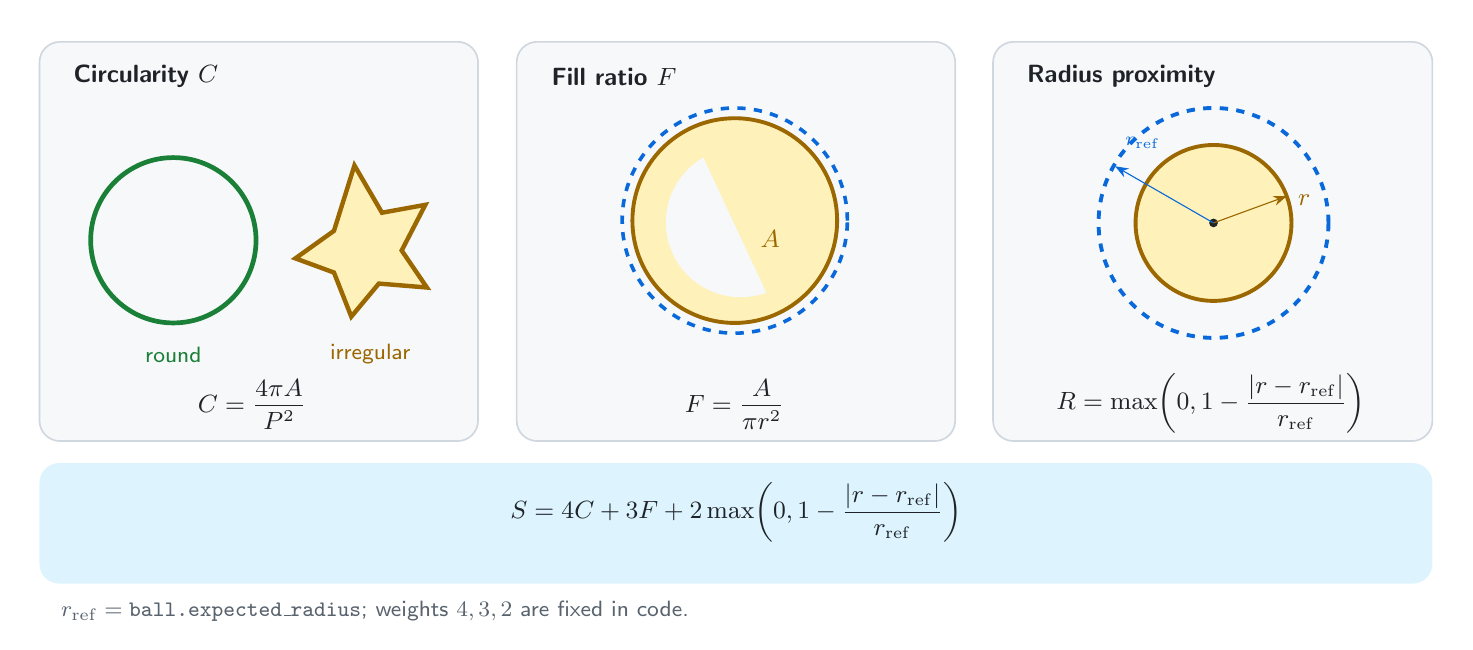
\begin{tikzpicture}[x=1cm, y=1cm]
        \path[use as bounding box] (0, 0) rectangle (18, 7.55);

        % Three components of the candidate score.
        \draw[card] (0.15, 2.3) rectangle (5.72, 7.37);
        \draw[card] (6.21, 2.3) rectangle (11.78, 7.37);
        \draw[card] (12.26, 2.3) rectangle (17.84, 7.37);

        \node[heading, anchor=west] at (0.46, 6.93) {Circularity $C$};
        \node[heading, anchor=west] at (6.53, 6.93) {Fill ratio $F$};
        \node[heading, anchor=west] at (12.57, 6.93) {Radius proximity};

        % Circular vs. irregular contours.
        \draw[ghgreen, line width=1.7pt] (1.85, 4.85) circle (1.05);
        \path[fill=ghorangesoft, draw=ghorange, line width=1.6pt]
            (4.15, 5.8) -- (4.5, 5.2) -- (5.05, 5.3)
            -- (4.75, 4.72) -- (5.07, 4.25) -- (4.46, 4.3)
            -- (4.11, 3.88) -- (3.89, 4.44) -- (3.4, 4.62)
            -- (3.89, 4.97) -- cycle;

        \node[note, text=ghgreen] at (1.85, 3.4) {round};
        \node[note, text=ghorange] at (4.35, 3.4) {irregular};
        \node[mathlabel] at (2.85, 2.77)
            {$C=\dfrac{4\pi A}{P^2}$};

        % Fraction of the enclosing circle filled by a contour.
        \begin{scope}[shift={(8.98, 5.1)}]
            \draw[ghblue, dashed, line width=1.3pt]
                (0, 0) circle (1.43);
            \fill[ghorangesoft] (0, 0) circle (1.3);
            \draw[ghorange, line width=1.4pt] (0, 0) circle (1.3);
            \path[fill=ghpanel]
                (-0.4, 0.8)
                arc[start angle=120, end angle=290, radius=0.95]
                -- cycle;
            \node[mathlabel, text=ghorange] at (0.45, -0.23) {$A$};
        \end{scope}

        \node[mathlabel] at (8.98, 2.77)
            {$F=\dfrac{A}{\pi r^2}$};

        % Observed radius versus the configured reference radius.
        \begin{scope}[shift={(15.06, 5.07)}]
            \draw[ghblue, dashed, line width=1.4pt]
                (0, 0) circle (1.46);
            \fill[ghorangesoft] (0, 0) circle (0.99);
            \draw[ghorange, line width=1.4pt] (0, 0) circle (0.99);
            \fill[ghtext] (0, 0) circle (0.055);
            \draw[ghblue, -Stealth] (0, 0) -- (-1.25, 0.72);
            \draw[ghorange, -Stealth] (0, 0) -- (0.93, 0.34);

            \node[tinylabel, text=ghblue, anchor=south]
                at (-0.9, 0.82) {$r_{\mathrm{ref}}$};
            \node[mathlabel, text=ghorange, anchor=west]
                at (0.95, 0.29) {$r$};
        \end{scope}

        \node[mathlabel] at (15.03, 2.78)
            {$R=\max\!\left(0,1-\dfrac{|r-r_{\mathrm{ref}}|}{r_{\mathrm{ref}}}\right)$};

        % Final score: fixed weights, configurable expected radius.
        \path[fill=ghbluesoft, rounded corners=2.5mm]
            (0.15, 0.49) rectangle (17.84, 2.02);
        \node[mathlabel] at (9, 1.39)
            {$\displaystyle S=4C+3F+2\max\!\left(0,1-\frac{|r-r_{\mathrm{ref}}|}{r_{\mathrm{ref}}}\right)$};
        \node[note, anchor=west] at (0.3, 0.14)
            {$r_{\mathrm{ref}}=\texttt{ball.expected\_radius}$; weights $4,3,2$ are fixed in code.};
    \end{tikzpicture}
\end{document}
